\documentclass[presentation]{beamer}

\usepackage[utf8]{inputenc}
% \usepackage[T1]{fontenc}
\usepackage{fixltx2e}
\usepackage{graphicx}
% \usepackage{longtable}
% \usepackage{tabu}
\usepackage{makecell}
\usepackage{float}
\usepackage{subcaption}
\usepackage{wrapfig}
\usepackage{rotating}
\usepackage[normalem]{ulem}
\usepackage{amsmath}
% \usepackage{textcomp}
% \usepackage{marvosym}
% \usepackage{wasysym}
% \usepackage{amssymb}
\usepackage{hyperref}
\usepackage{ragged2e}

\usepackage{bm}

\usepackage{amsmath,amssymb}
\newcommand{\bx}{\mathbf{x}}
\newcommand{\bv}{\mathbf{v}}
\newcommand{\bp}{\mathbf{p}}
\newcommand{\bq}{\mathbf{q}}
\newcommand{\by}{\mathbf{y}}

\newcommand{\bbR}{\mathbb{R}}
\newcommand{\bbN}{\mathbb{N}}

\newcommand{\bxi}{\bm{\xi}}
\newcommand{\bal}{\bm{\alpha}}
\newcommand{\bth}{\bm{\theta}}

\usepackage{etoolbox}
\let\bbordermatrix\bordermatrix
\patchcmd{\bbordermatrix}{8.75}{4.75}{}{}
\patchcmd{\bbordermatrix}{\left(}{\left[}{}{}
\patchcmd{\bbordermatrix}{\right)}{\right]}{}{}

\usepackage[authoryear, round]{natbib}

\newcommand{\sidebysidecaption}[4]{%
\RaggedRight%
  \begin{minipage}[t]{#1}
    \vspace*{0pt}
    #3
  \end{minipage}
  \hfill%
  \begin{minipage}[t]{#2}
    \vspace*{0pt}
    #4
\end{minipage}%
}

%% colors
\definecolor{Red}{rgb}{0.7,0,0}
\definecolor{Blue}{rgb}{0,0,0.8}
\definecolor{Green}{rgb}{0,0.8,0}
\definecolor{Gray}{rgb}{0.8,0.8,0.8}
\definecolor{Orange}{rgb}{1,.65,0}

\usepackage{hyperref}
\hypersetup{
  hyperindex = {true},
  colorlinks = {true},
  linktocpage = {true},
  plainpages = {false},
  linkcolor = {Blue},
  citecolor = {Blue},
  urlcolor = {Red},
  pdfstartview = {Fit},
  pdfpagemode = {UseOutlines},
  pdfview = {XYZ null null null},
  pdfkeywords={proteomics, spatial, dynamics, integration, regulation, computational biology},
  pdfsubject={Research talk},
  pdfcreator={Laurent Gatto}}

\date{26 September 2018, Gent}

\title{
  \textbf{Mapping the sub-cellular proteome}
}

\author{Laurent Gatto\\
  \url{laurent.gatto@uclouvain.be} -- \url{@lgatt0}\\
  de Duve Institute -- UCLouvain\\
  \url{http://lgatto.github.io/about}\\
  \bigskip
  Slides: %%  \includegraphics[height=3mm]{./figs_local/zenodo1180393.png}\\
  \url{TODO}
}


% \AtBeginSection[] % Do nothing for \section*
% {
%   \begin{frame}<beamer>
%     \frametitle{Plan}
%     \tableofcontents[currentsection]
%   \end{frame}
% }


\begin{document}

\maketitle

% \begin{frame}{}
%   Who?
% \end{frame}


\section{Spatial proteomics}

\subsection{The LOPIT pipeline}

\subsection*{Introduction}


\label{sec:spspatprot}

\begin{frame}{Cell organisation}
  \begin{center}
    \includegraphics[width=1\linewidth]{Figures/Animal_cell_structure.png} \\
    \textbf{\textcolor{Blue}{Spatial proteomics}} is the systematic
    study of protein localisations.
  \end{center}

  \tiny Image from Wikipedia
  \url{http://en.wikipedia.org/wiki/Cell_(biology)}.
\end{frame}

\begin{frame}{Regulations}
  \begin{figure}[h]
    \centering
    \includegraphics[width=1\linewidth]{Figures2/regulation.jpg}
  \end{figure}
\end{frame}

\begin{frame}{Spatial proteomics - Why?}
  \begin{block}{Localisation is function}
    \begin{itemize}
    \item The cellular sub-division allows cells to establish a range
      of distinct micro-environments, each favouring different
      biochemical reactions and interactions and, therefore, allowing
      each compartment to fulfil a particular functional role.
    \item Localisation and sequestration of proteins within
      sub-cellular niches is a fundamental mechanism for the
      post-translational regulation of protein function.
    \end{itemize}
  \end{block}
  \begin{block}{Re-localisation in}
    \begin{itemize}
    \item \textcolor{Blue}{Differentiation} stem cells.
    \item \textcolor{Blue}{Activation} of biological processes.
    \end{itemize}
    Examples later.
  \end{block}
\end{frame}

\begin{frame}{Spatial proteomics - Why?}
  \begin{block}{Mis-localisation}
    Disruption of the targeting/trafficking process alters proper
    sub-cellular localisation, which in turn perturb the cellular
    functions of the proteins.
    \begin{itemize}
    \item Abnormal protein localisation leading to the \textbf{loss of
        functional} effects in diseases \citep{Laurila2009}.
    \item Disruption of the nuclear/cytoplasmic transport (nuclear
      pores) have been detected in many types of \textbf{carcinoma
        cells} \citep{Kau2004}.
    \item Sub-cellular localisation of MC4R with ADCY3 at neuronal
      primary cilia underlies a common pathway for genetic
      predisposition to \textbf{obesity} \citep{Siljee:2018}.
    \end{itemize}
  \end{block}

\end{frame}


\subsubsection*{Experimental designs}
\label{sec:expdesign}

\begin{frame}{Spatial proteomics - How, experimentally}
  \begin{figure}
    \includegraphics[width=.8\linewidth]{Figures/F02-expdesigns.pdf}
    \caption{Organelle proteomics approaches \citep{Gatto:2010}}
  \end{figure}
\end{frame}


% \begin{frame}{Microscopy}
%   \begin{columns}[t]
%     \begin{column}[T]{0.5\textwidth}
%       \begin{figure}
%         \includegraphics[width=.7\linewidth]{Figures2/Localisations02eng.jpg}
%         \caption{\textbf{Fluorescent protein fusion} localisation of
%         proteins using GFP tagging. (from Wikipedia)}
%       \end{figure}
%     \end{column}
%     \begin{column}[T]{0.49\textwidth}
%       \begin{centering}
%         \begin{figure}
%           \includegraphics[width=.49\linewidth]{Figures2/172H11blueredgreen.jpg}
%           \includegraphics[width=.49\linewidth]{Figures2/34C71blueredgreen.jpg}
%           \caption{\textbf{Immunofluorescence}: ZFPL1, GO (left) and FHL2, mainly localized to
%           actin filaments and focal adhesion sites. Also detected in
%           the nucleus (right). (from the Human Protein Atlas)}
%         \end{figure}
%       \end{centering}
%     \end{column}
%   \end{columns}
% \end{frame}

\begin{frame}{Fusion proteins and immunofluorescence}

  \begin{figure}[h]
    \centering
    \includegraphics[width=.35\linewidth]{Figures2/Localisations02eng.jpg}
    \includegraphics[width=.45\linewidth]{figures/if_selected.jpg}
    \caption{Targeted protein localisation. Example of discrepancies
      between IF and FPs as well as between FP tagging at the N and C
      termini \citep{Stadler:2013}.}
  \end{figure}
\end{frame}

% \begin{frame}{Fusion proteins and immunofluorescence}
%   \begin{figure}
%     \centering
%     \includegraphics[angle=-90, width=.8\linewidth]{Figures2/Disc-IF-IP.png} \\
%     \includegraphics[angle=-90, width=.8\linewidth]{Figures2/Disc-N-C.png}
%     \caption{Example of discrepancies between IF and FPs as well as
%       between FP tagging at the N and C termini (Stadler et al., 2013).}
%   \end{figure}
% \end{frame}

\subsubsection*{Gradient approaches}
\label{sec:grad}

\begin{frame}{Spatial proteomics - How, experimentally}
  \begin{figure}
    \includegraphics[width=.8\linewidth]{Figures/F02-expdesigns.pdf}
    \caption{Organelle proteomics approaches
      \citep{Gatto:2010}.}
  \end{figure}

  \textbf{Gradient approaches}: \cite{Dunkley:2006},
  \cite{Foster2006}, based on works by de Duve, Claude and Palade.

  \bigskip

  \textbf{Explorative/discovery approaches},
  \textcolor{Blue}{steady-state \textbf{global localisation maps}}.
\end{frame}


\begin{frame}{}
  \begin{figure}
    % \includegraphics[width=.8\linewidth]{Figures/F03-protocols-8plex.pdf}
    % \includegraphics[width=.5\linewidth]{figures/expdesign.pdf}
    \includegraphics[width=.39\linewidth]{figures/workflow_primary.pdf}
  \end{figure}
\end{frame}

\subsubsection*{The data}
\label{sec:data}

\begin{frame}{Quantitation data}
  \begin{center}
    \begin{tabular}{|l|llll|}
      \hline
      & Fraction$_{\text{1}}$ & Fraction$_{\text{2}}$ & \ldots{} & Fraction$_{\text{m}}$ \\
      \hline
      p$_{\text{1}}$ & q$_{\text{1,1}}$ & q$_{\text{1,2}}$ & \ldots{} & q$_{\text{1,m}}$ \\
      p$_{\text{2}}$ & q$_{\text{2,1}}$ & q$_{\text{2,2}}$ & \ldots{} & q$_{\text{2,m}}$ \\
      p$_{\text{3}}$ & q$_{\text{3,1}}$ & q$_{\text{3,2}}$ & \ldots{} & q$_{\text{3,m}}$ \\
      p$_{\text{4}}$ & q$_{\text{4,1}}$ & q$_{\text{4,2}}$ & \ldots{} & q$_{\text{4,m}}$ \\
      \vdots & \vdots & \vdots & \vdots & \vdots \\
      p$_{\text{j}}$ & q$_{\text{j,1}}$ & q$_{\text{j,2}}$ & \ldots{} & q$_{\text{j, m}}$  \\
      \hline
    \end{tabular}
  \end{center}
\end{frame}

\begin{frame}{Quantitation data and organelle markers}
  \begin{center}
    \begin{tabular}{|l|llll||l|}
      \hline
      & Fraction$_{\text{1}}$ & Fraction$_{\text{2}}$ & \ldots{} & Fraction$_{\text{m}}$ & markers\\
      \hline
      p$_{\text{1}}$ & q$_{\text{1,1}}$ & q$_{\text{1,2}}$ & \ldots{} & q$_{\text{1,m}}$ & unknown \\
      p$_{\text{2}}$ & q$_{\text{2,1}}$ & q$_{\text{2,2}}$ & \ldots{} & q$_{\text{2,m}}$ & \textcolor{Red}{$loc_{1}$}\\
      p$_{\text{3}}$ & q$_{\text{3,1}}$ & q$_{\text{3,2}}$ & \ldots{} & q$_{\text{3,m}}$ & unknown \\
      p$_{\text{4}}$ & q$_{\text{4,1}}$ & q$_{\text{4,2}}$ & \ldots{} & q$_{\text{4,m}}$ & \textcolor{Blue}{$loc_{i}$}\\
      \vdots & \vdots & \vdots & \vdots & \vdots & \vdots\\
      p$_{\text{j}}$ & q$_{\text{j,1}}$ & q$_{\text{j,2}}$ & \ldots{} & q$_{\text{j, m}}$ & unknown \\
      \hline
    \end{tabular}
  \end{center}
\end{frame}

\subsection*{Data analysis}
\label{sec:comp}


\begin{frame}{Data analysis}
  \begin{itemize}
  \item Visualisation (unsupervised learning, clustering) \citep{Gatto:2018}
  \item Classification (supervised learning) \citep{Breckels:2016b}
  \item Novelty detection (semi-supervised learning) \cite{Breckels:2013}
  \item Data integration (transfer learning) \citep{Breckels:2016}
  \item Probabilistic modelling \citep{Crook:2018}
  \end{itemize}
\end{frame}



\subsubsection*{Visualisation}
\label{sec:viz}

\begin{frame}{Visualisation}
  \begin{figure}
    \centering
    \includegraphics[width=.6\linewidth]{Figures/F04-analyses.pdf}
    \caption{From \cite{Gatto:2010}, \textit{Arabidopsis thaliana} data
      from \cite{Dunkley:2006}}
  \end{figure}
\end{frame}

\subsubsection*{Machine learning}
\label{sec:ml}


\begin{frame}{Supervised Machine Learning}
  \begin{figure}[h]
    \centering
    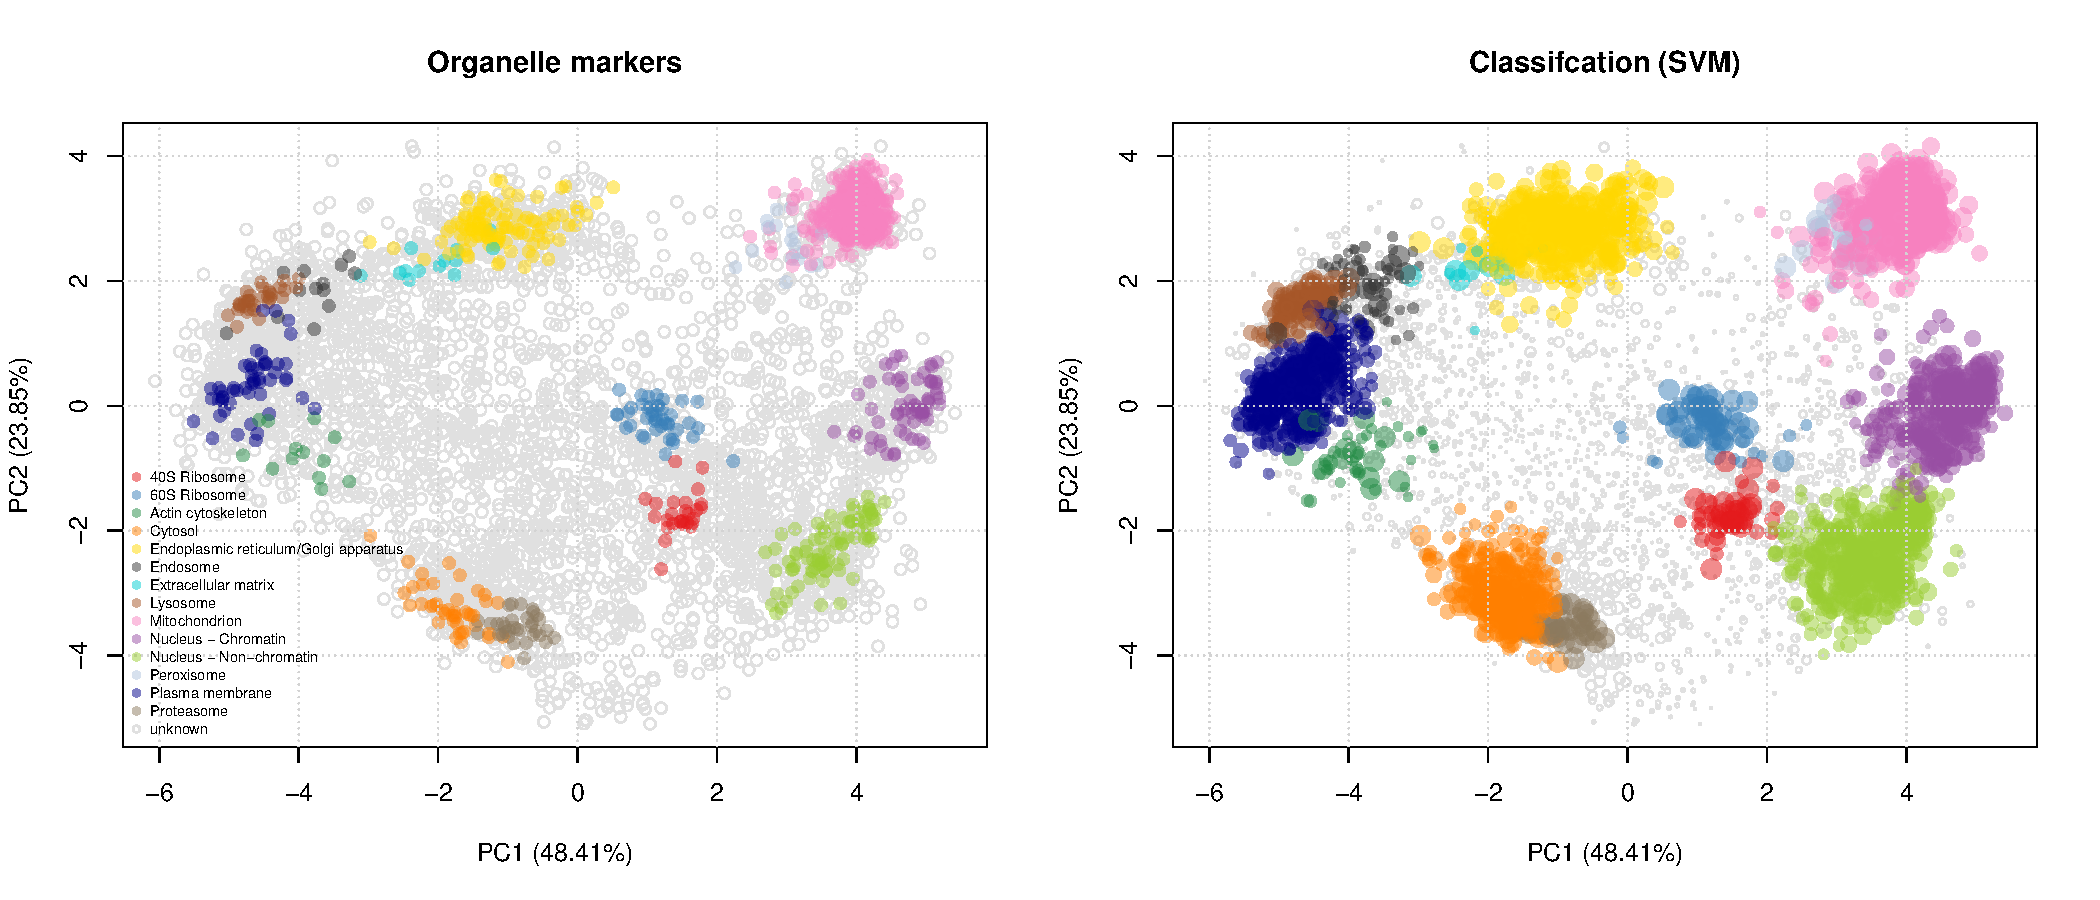
\includegraphics[width=\linewidth]{figs_local/hyperlopit-class.pdf}
    \caption{Support vector machines classifier (after 5\% FDR
      classification cutoff) on the embryonic stem cell data from
      \cite{Christoforou:2016}.}
  \end{figure}
\end{frame}


\begin{frame}{Importance of annotation}
  \begin{columns}[t]
    \begin{column}[T]{0.43\textwidth}
      \begin{centering}
        \includegraphics[width=1\linewidth]{Figures/tan2009r1org.pdf}
      \end{centering}
    \end{column}
    \begin{column}[T]{0.56\textwidth}
      \includegraphics[width=1\linewidth]{Figures/Animal_cell_structure.png}
    \end{column}
  \end{columns}
  Incomplete annotation, and therefore lack of training data, for
  many/most organelles. \textit{Drosophila} data from \cite{Tan2009}.
\end{frame}

\begin{frame}{Semi-supervised learning: novelty detection}
  \begin{figure}
    \includegraphics[width=.48\linewidth]{Figures/tan2009r1org.pdf}
    \includegraphics[width=.5\linewidth]{Figures/pdres2fig.pdf}
    \caption{Left: Original \textit{Drosophila} data from
      \cite{Tan2009}. Right: After semi-supervised learning and
      classification, \cite{Breckels:2013}.}
  \end{figure}
\end{frame}

\subsection{Biological applications}

%% NOTES: what I have presented so far has been state-of-the art since
%% about 2016. Except for the transfer learning, that I didn't
%% present, the efforts have been very descriptive, with relatively
%% little advanced biological inference from the data. What I am going
%% to present now allows, in my opinion, a much deeper dive into the
%% data and a much more thorough understanding of the biology
%% described by these data.

\begin{frame}{Biological discoveries}
  \begin{itemize}
  \item Multi-localisation (embracing uncertainty, probabilistic
    modelling)
  \item Trans-localisation
  \end{itemize}
\end{frame}

\subsection{Embracing uncertainty}

\begin{frame}{A Bayesian Mixture Modelling Approach For Spatial Proteomics}

  \begin{itemize}

    \item<+-> \textit{T Augmented Gaussian Mixture model (TAGM)} is a
      \textbf{multivariate Gaussian generative model} for MS-based
      spatial proteomics data. It posits that each annotated
      sub-cellular niche can be modelled by a multivariate Gaussian
      distribution.

    \item<+-> With the prior knowledge that many proteins are not
      captured by known sub-cellular niches, we augment our model with
      an outlier component. Outliers are often dispersed and thus this
      additional component is described by a heavy-tailed
      distribution: the multivariate Student's t-distribution, leading
      us to a T Augmented Gaussian Mixture model (TAGM) .

    \item<+-> This methodology allows proteome-wide
      \textbf{uncertainty quantification}, thus adding a further layer
      to the analysis of spatial proteomics.

  \end{itemize}
\end{frame}

\begin{frame}[fragile]{}
      \begin{figure}
        \sidebysidecaption{0.65\linewidth}{0.3\linewidth}{
          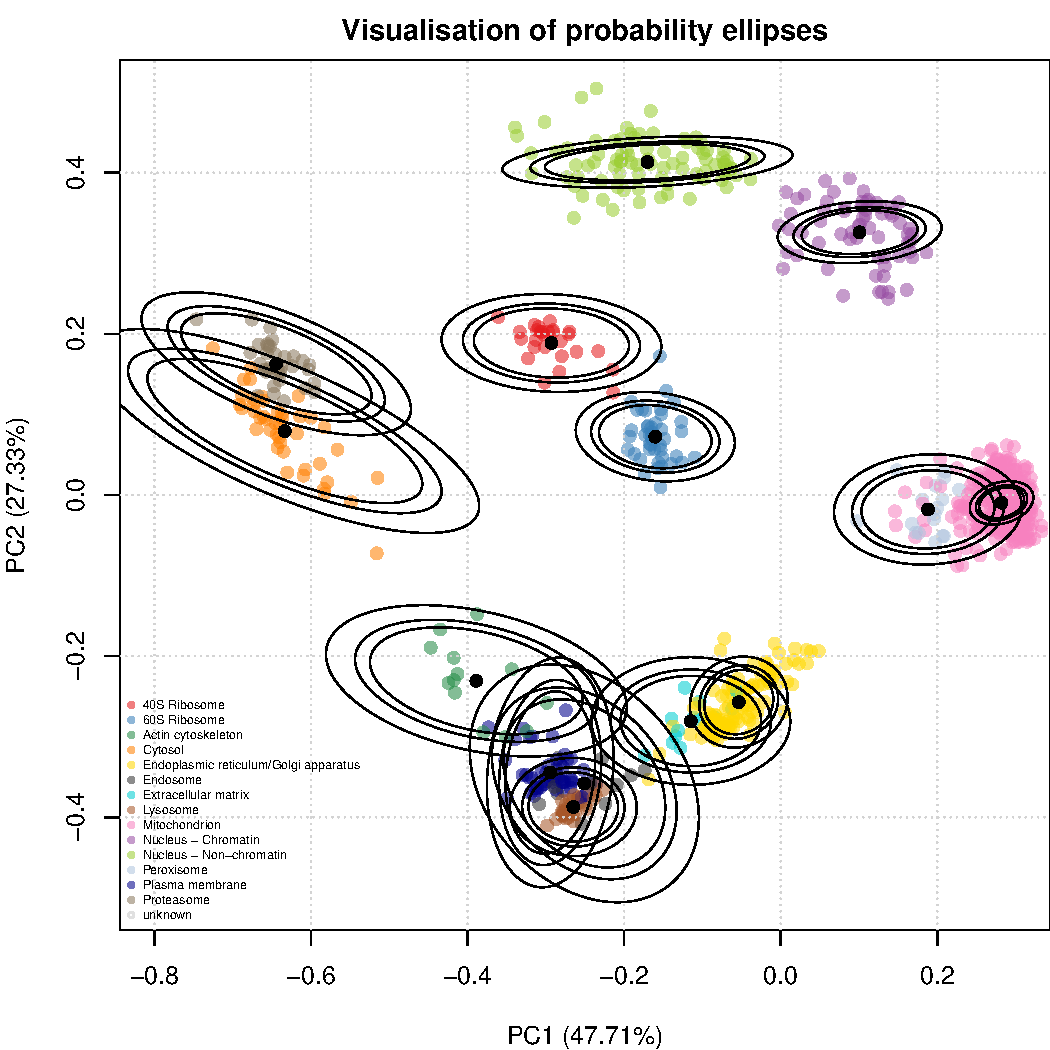
\includegraphics[width=1\linewidth]{./figs_local/pca12-ellipses-1.pdf}
        }{
          \caption{\scriptsize \justifying Illustration of how the
            TAGM model describes the pluripotent mouse embryonic stem
            cell data. Each ellipse contains a proportion of total
            probability of a particular multivariate Gaussian density.
            The outer ellipse contains $99\%$ of the total probability
            whilst the middle and inner ellipses contain $95\%$ and
            $90\%$ of the probability respectively.}
          \label{fig:tagm}
        }
      \end{figure}

      %% NOTE that while some sub-cellular clusters overlap along PC1 and
      %% PC2, they are separated along additional dimensions.

\end{frame}

\begin{frame}{}
      \begin{figure}
        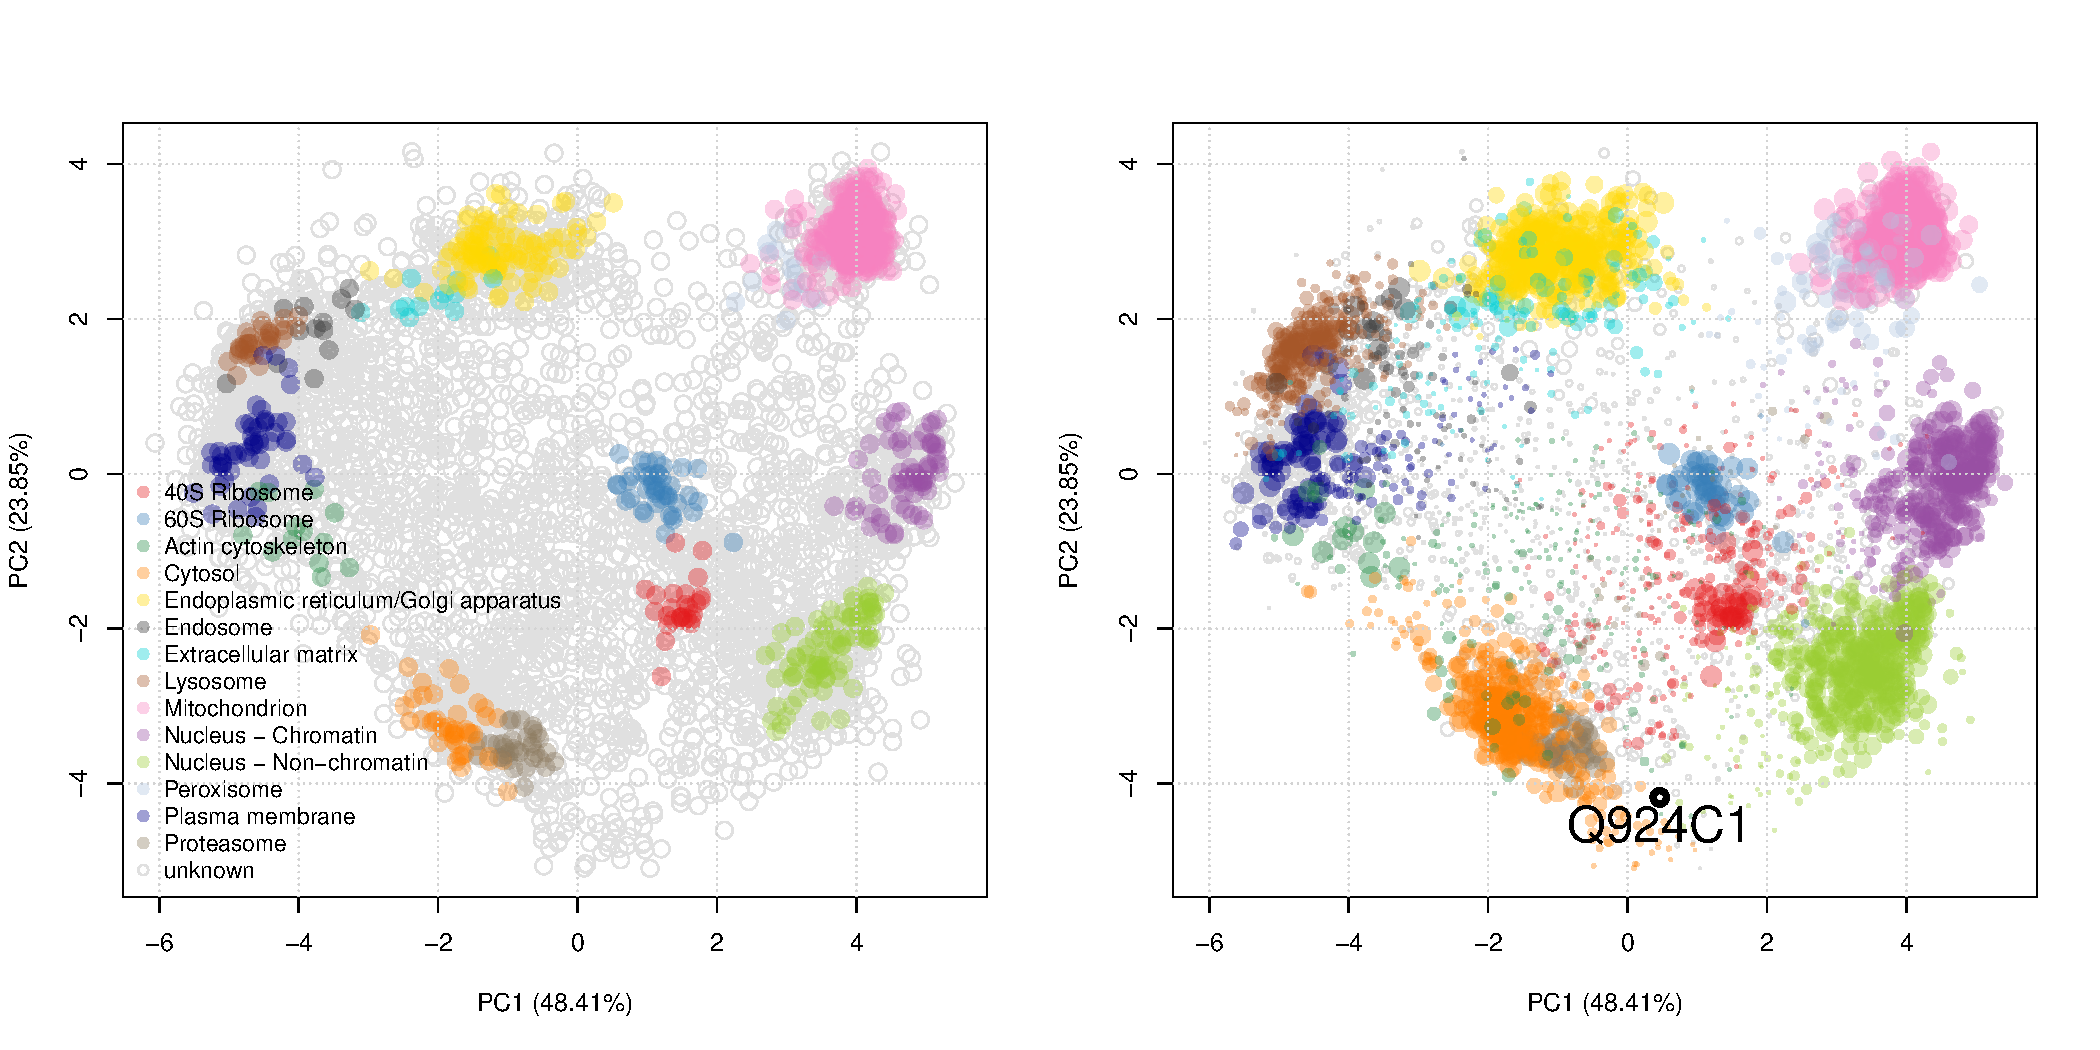
\includegraphics[width=1\linewidth]{./figs_local/pca.pdf}
        \caption{Assignment of proteins of
          \textit{unknown} location to one of the annotated
          classes. The dots are scaled according to the protein
          assignment probabilities.}
      \end{figure}
\end{frame}

\begin{frame}{}
  \begin{figure}
    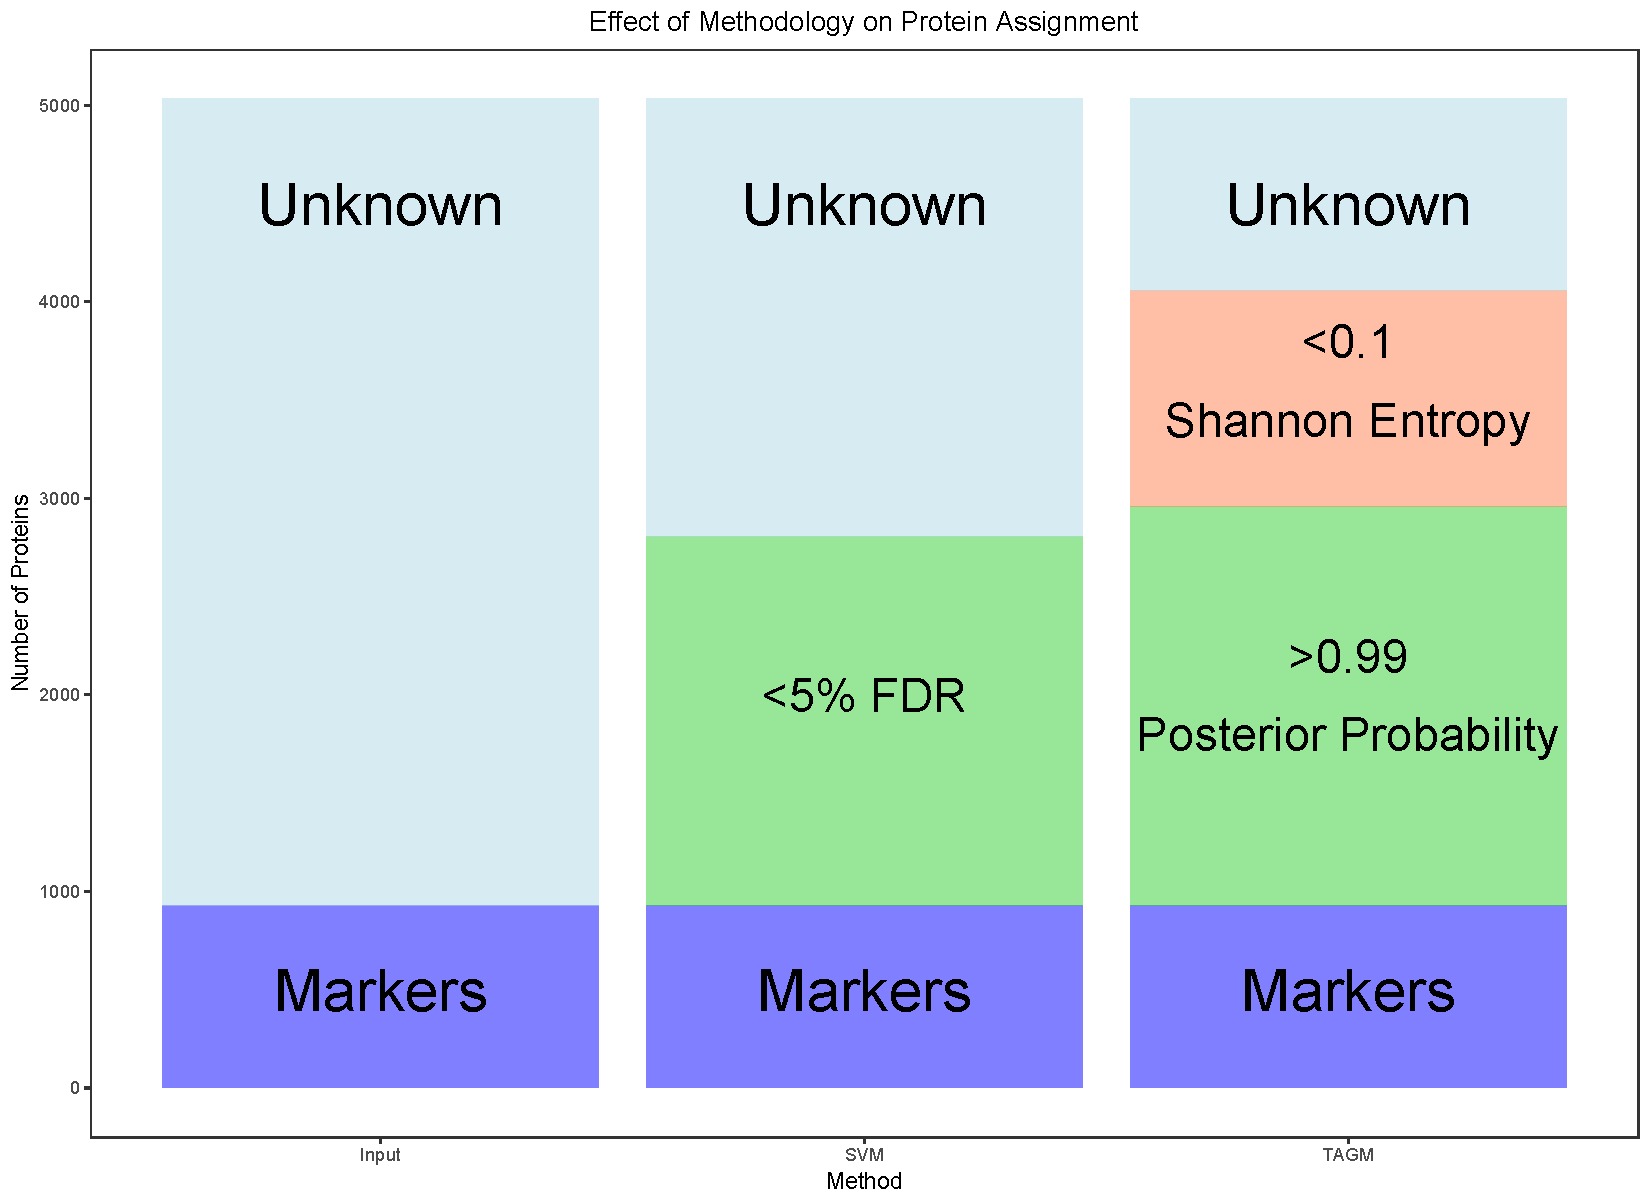
\includegraphics[width=.8\linewidth]{./figs_local/ConcludePlot.pdf}
  \end{figure}
\end{frame}

\begin{frame}
  \begin{figure}
    \centering
    \sidebysidecaption{0.55\linewidth}{0.42\linewidth}{
      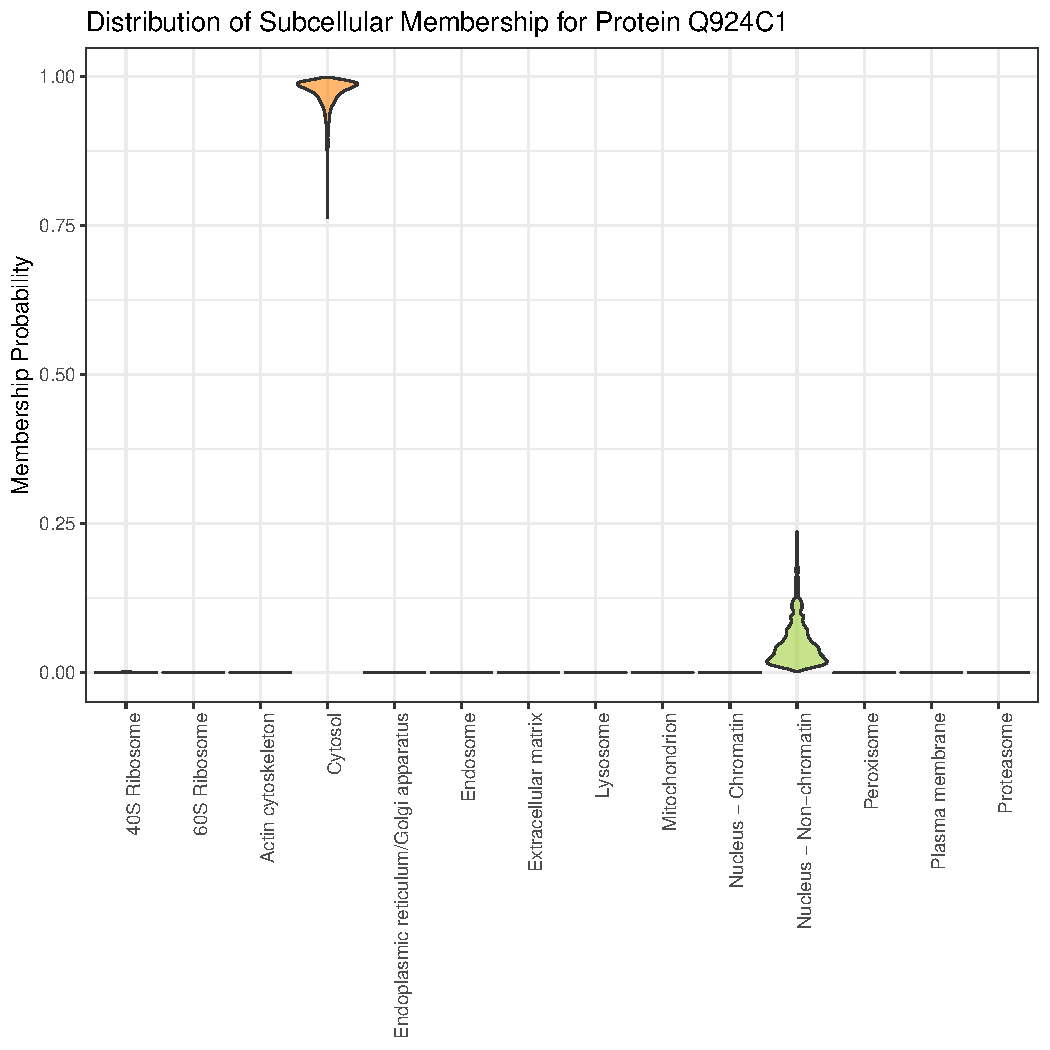
\includegraphics[width=1\linewidth]{./figs_local/Q924C1-prob-1.pdf}
    }{
    \caption{\scriptsize \justifying Exportin 5 (Q924C1) forms part of
      the micro-RNA export machinery of the nucleus, transporting
      miRNA from the nucleus to the cytoplasm for further processing.
      It then translocates back through the nuclear pore complex to
      return to the nucleus to mediate further transport between
      nucleus and cytoplasm. The model correctly infers that it most
      likely localises to the cytosol but there is some uncertainty
      with this assignment. This uncertainty is reflected in possible
      assignment of Exportin 5 to the nucleus non-chromatin and
      reflects the multi-location of the protein.}  }
    %% NOTE SVM failed to classify exportin 5 to any of the two
    %% biologically plausible locations, arguably due to the similarity
    %% of the cytosol and peroxysome, to which it got assigned.

  \end{figure}
\end{frame}

\begin{frame}{}
  \begin{figure}
    \centering
    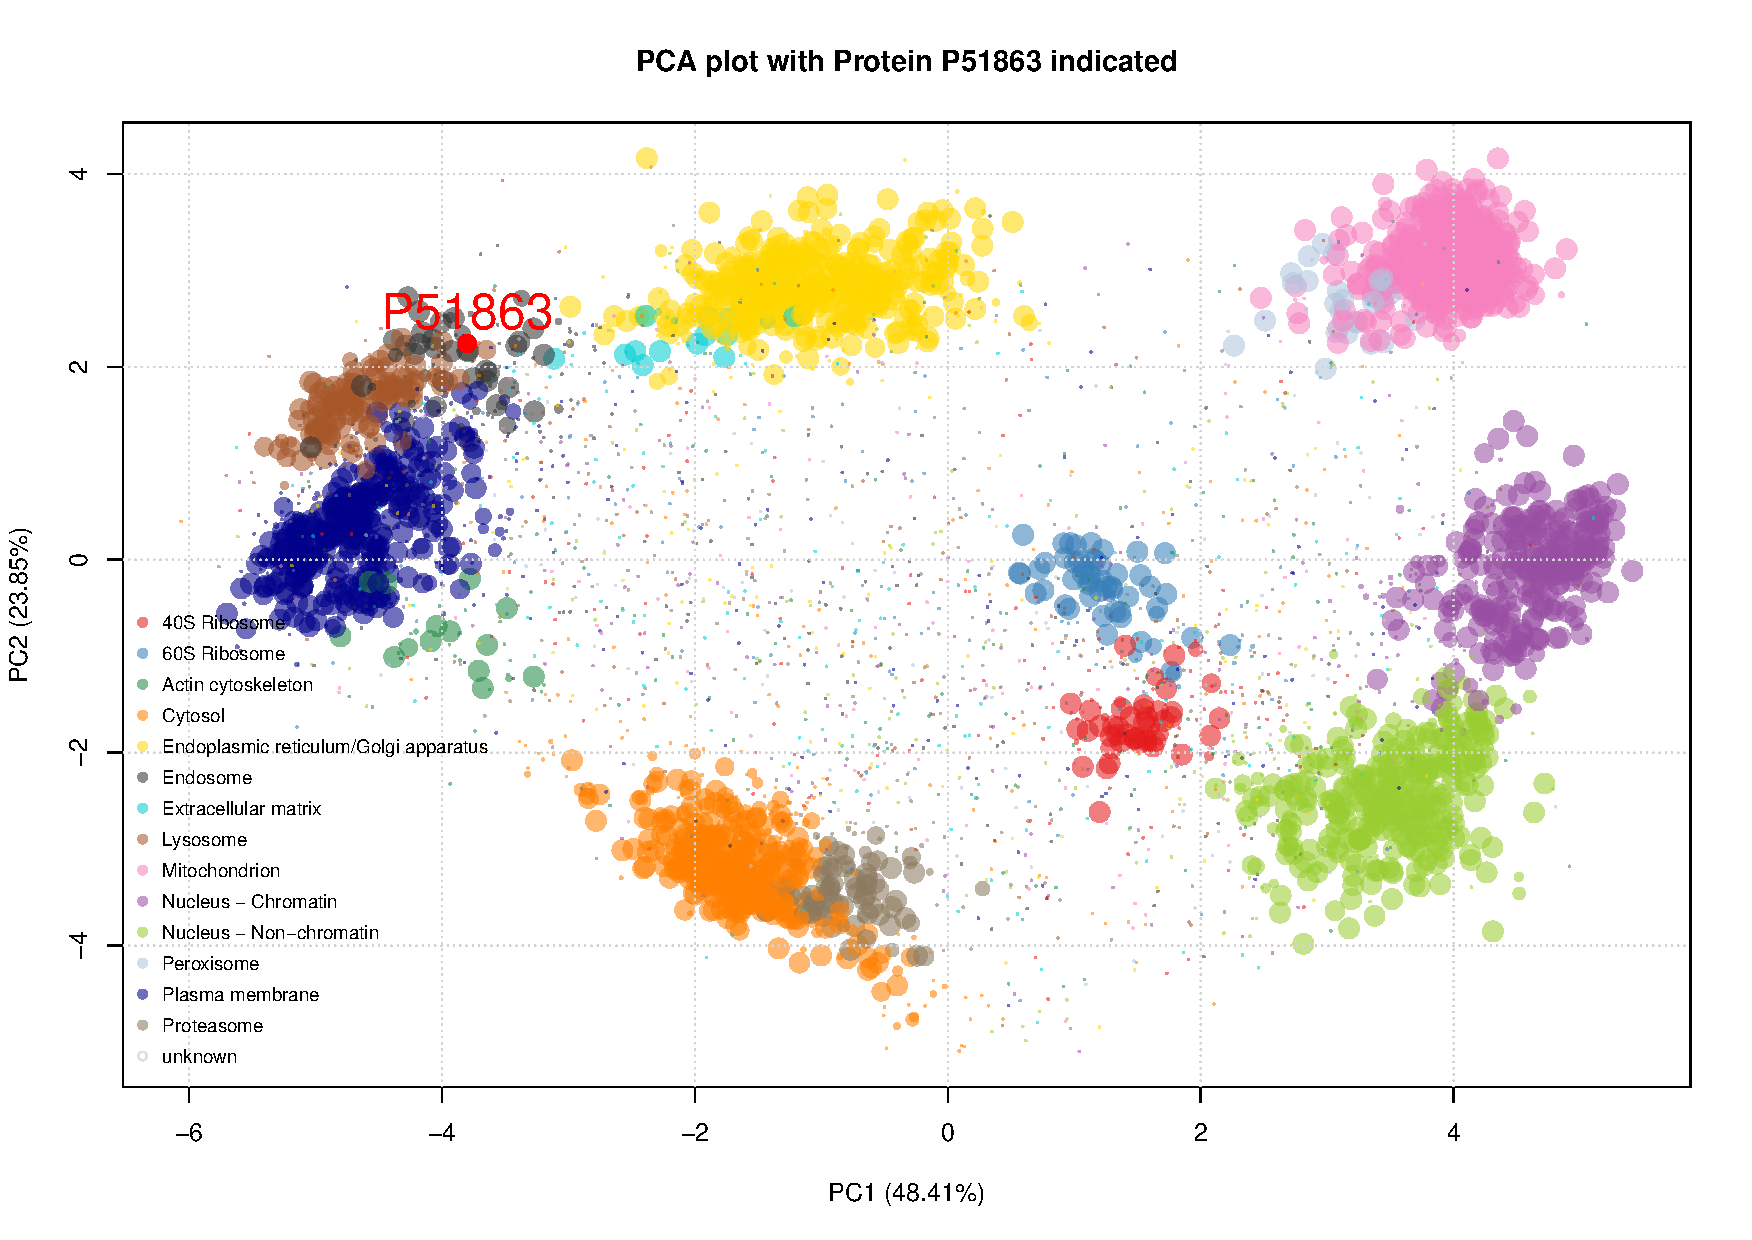
\includegraphics[width=.53\linewidth]{./figs_local/PCAP51863.pdf}
    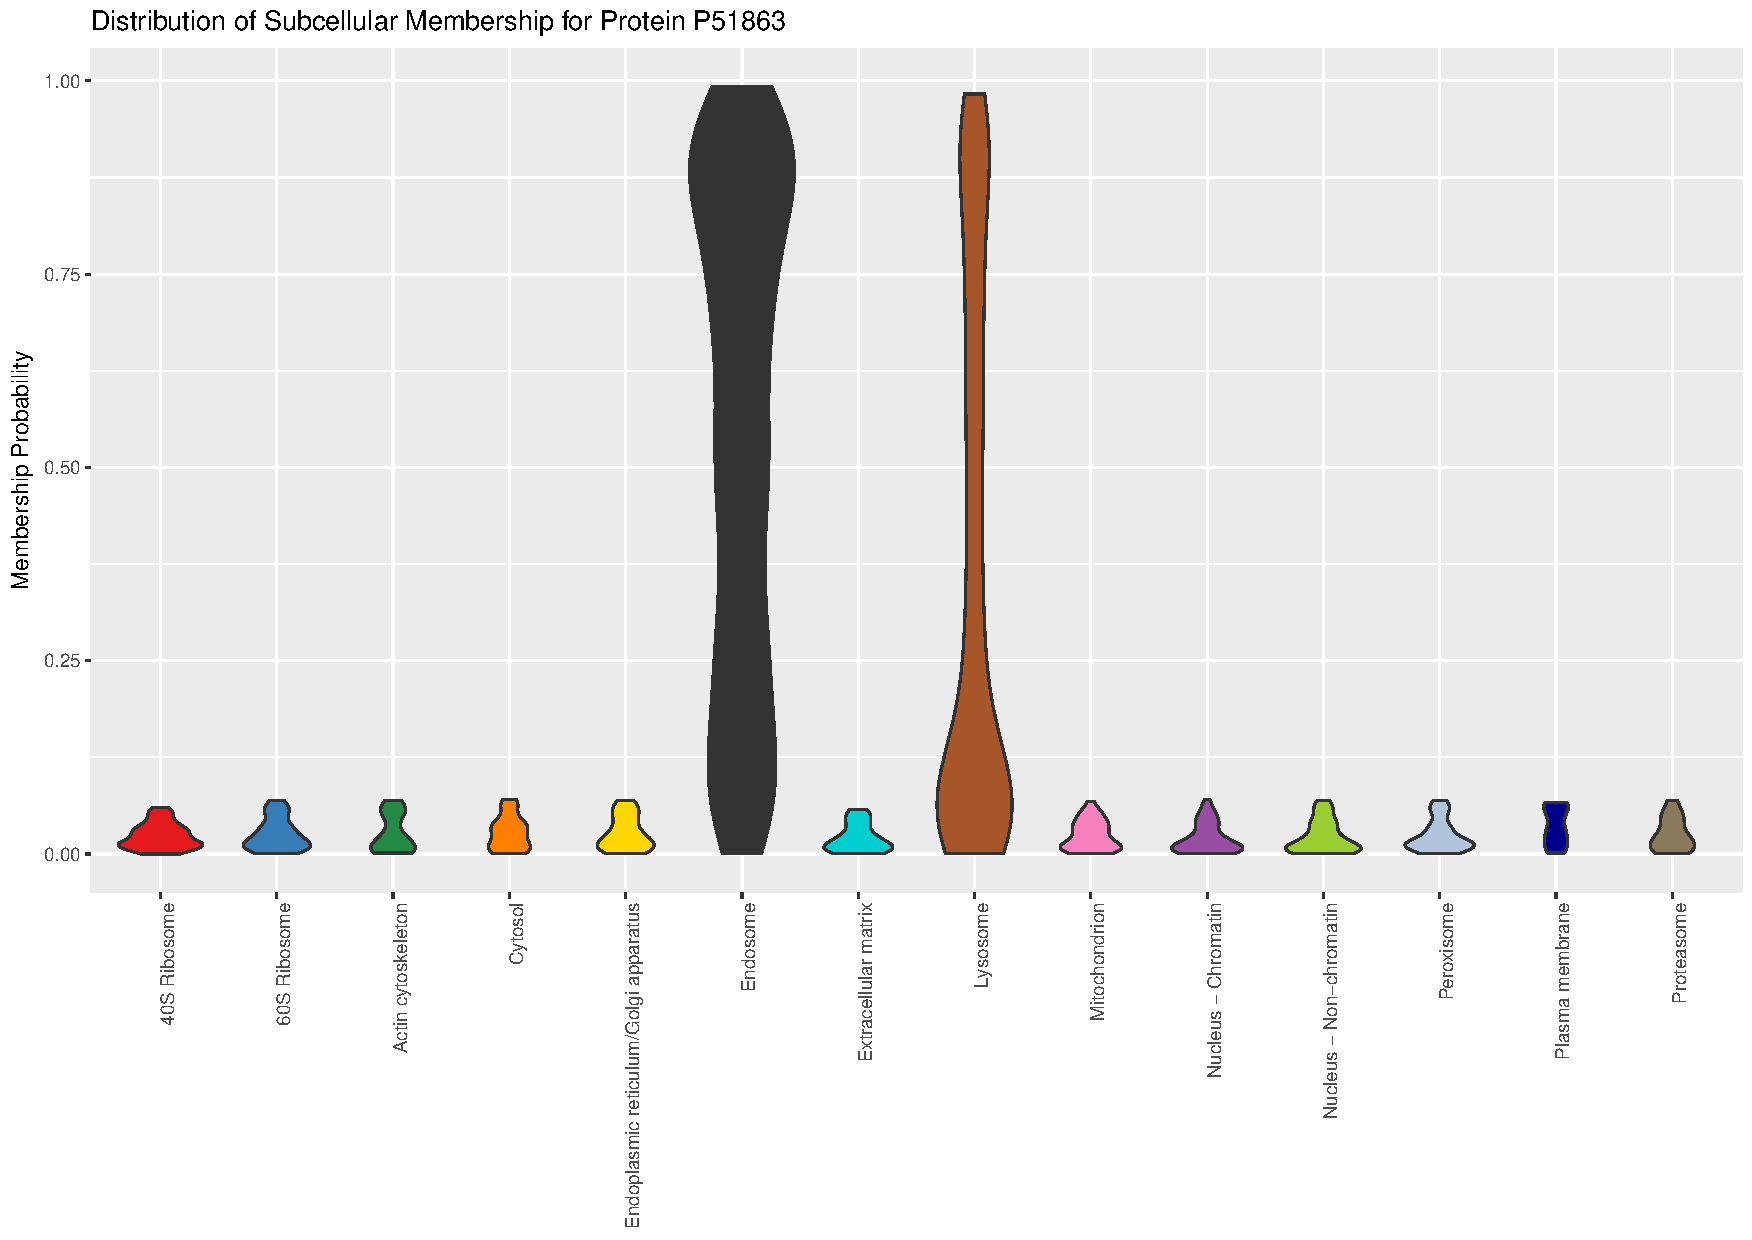
\includegraphics[width=.46\linewidth]{./figs_local/violinp51863.pdf}
    \caption{V-ATPase subunit d1 (P51683) with uncertain localisation
      between the endosome and lysosome.  }
  \label{fig:bgmm}
  \end{figure}
\end{frame}

\subsubsection{Trans-localisation}

\begin{frame}{Spatial dynamics}
  \begin{block}{Trans-localisation event during monocyte to macrophage
      differentiation}
    Investigate the effect of lipopolysaccharides (LPS)-mediated
    inflammatory response in human monocytic cells (THP-1)
  \end{block}

  \begin{block}{Data}
    \begin{itemize}
    \item Triplicate \textbf{temporal} profiling (0, 2, 4, 6, 12, 24
      hours).
    \item Triplicate \textbf{spatial} profiling (0 vs 12 hours) -
      early trafficking, before actual morphological differentiation
      at 24h.
    \end{itemize}
  \end{block}

  With \textbf{Dr Claire Mulvey} at the Cambridge Centre for
  Proteomics, now at CRUK Cambridge Institute.

\end{frame}



\begin{frame}
  \begin{figure}[h]
    \centering
    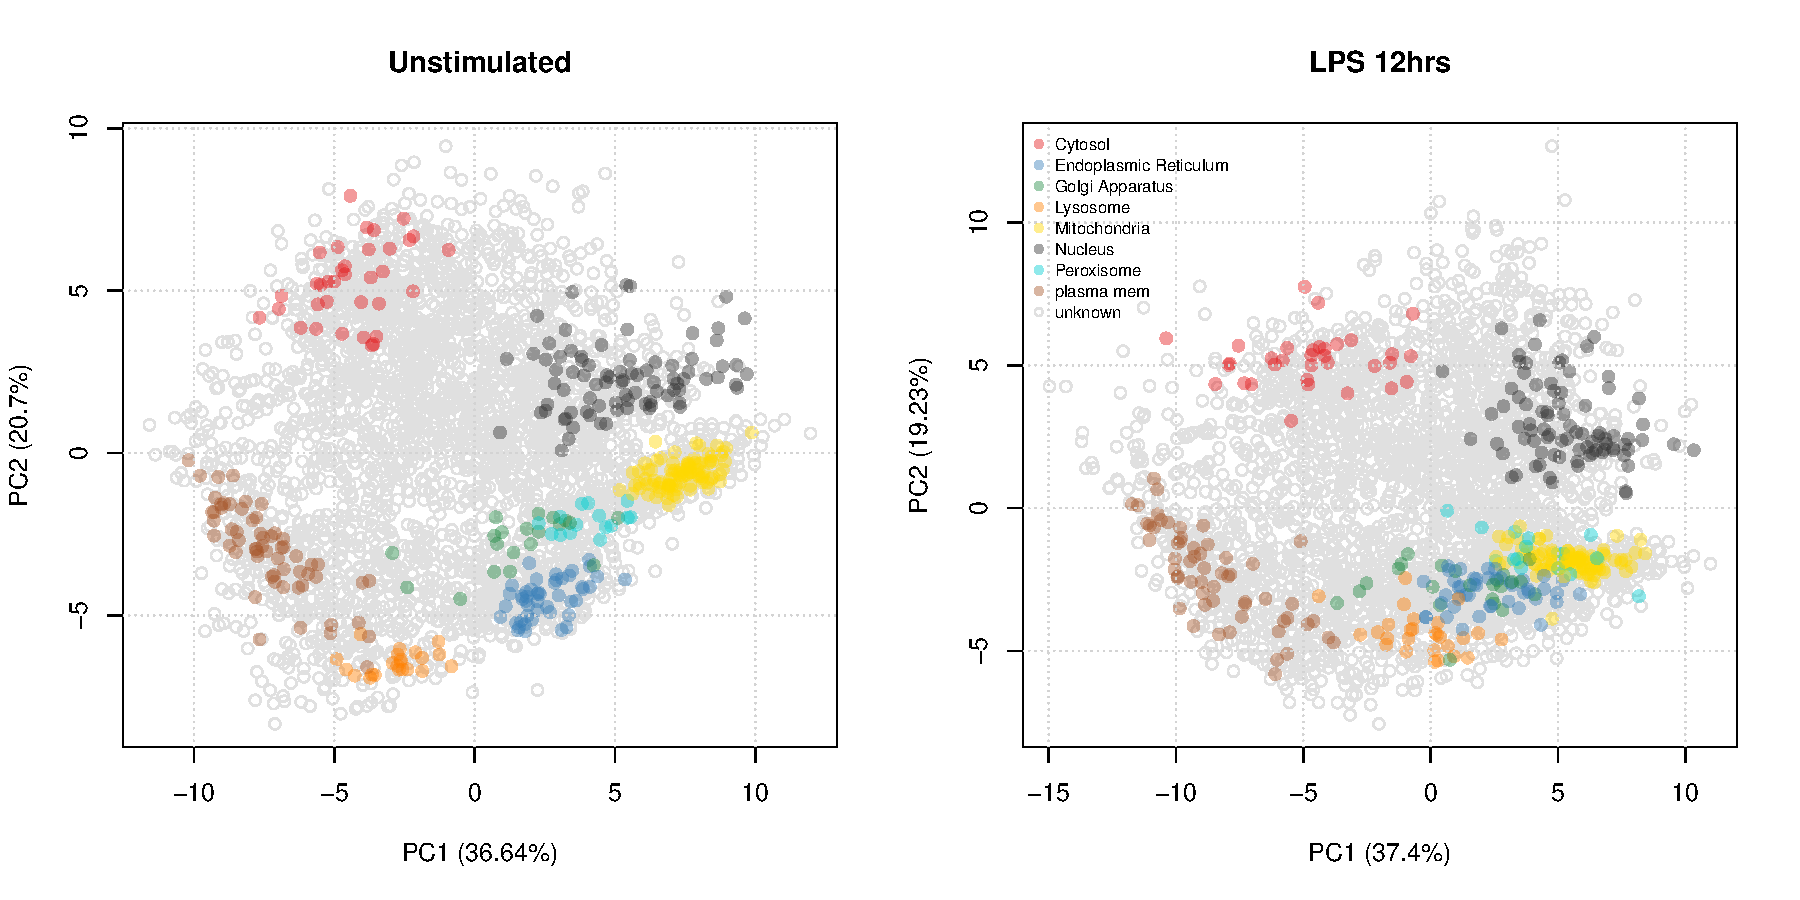
\includegraphics[width=\linewidth]{./figs_local/lps.pdf}
    \caption{Spatial maps of unstimulated and LPS-treated cells
      (combined triplicates).}
  \end{figure}
\end{frame}

\begin{frame}
  \begin{figure}[h]
    \centering
    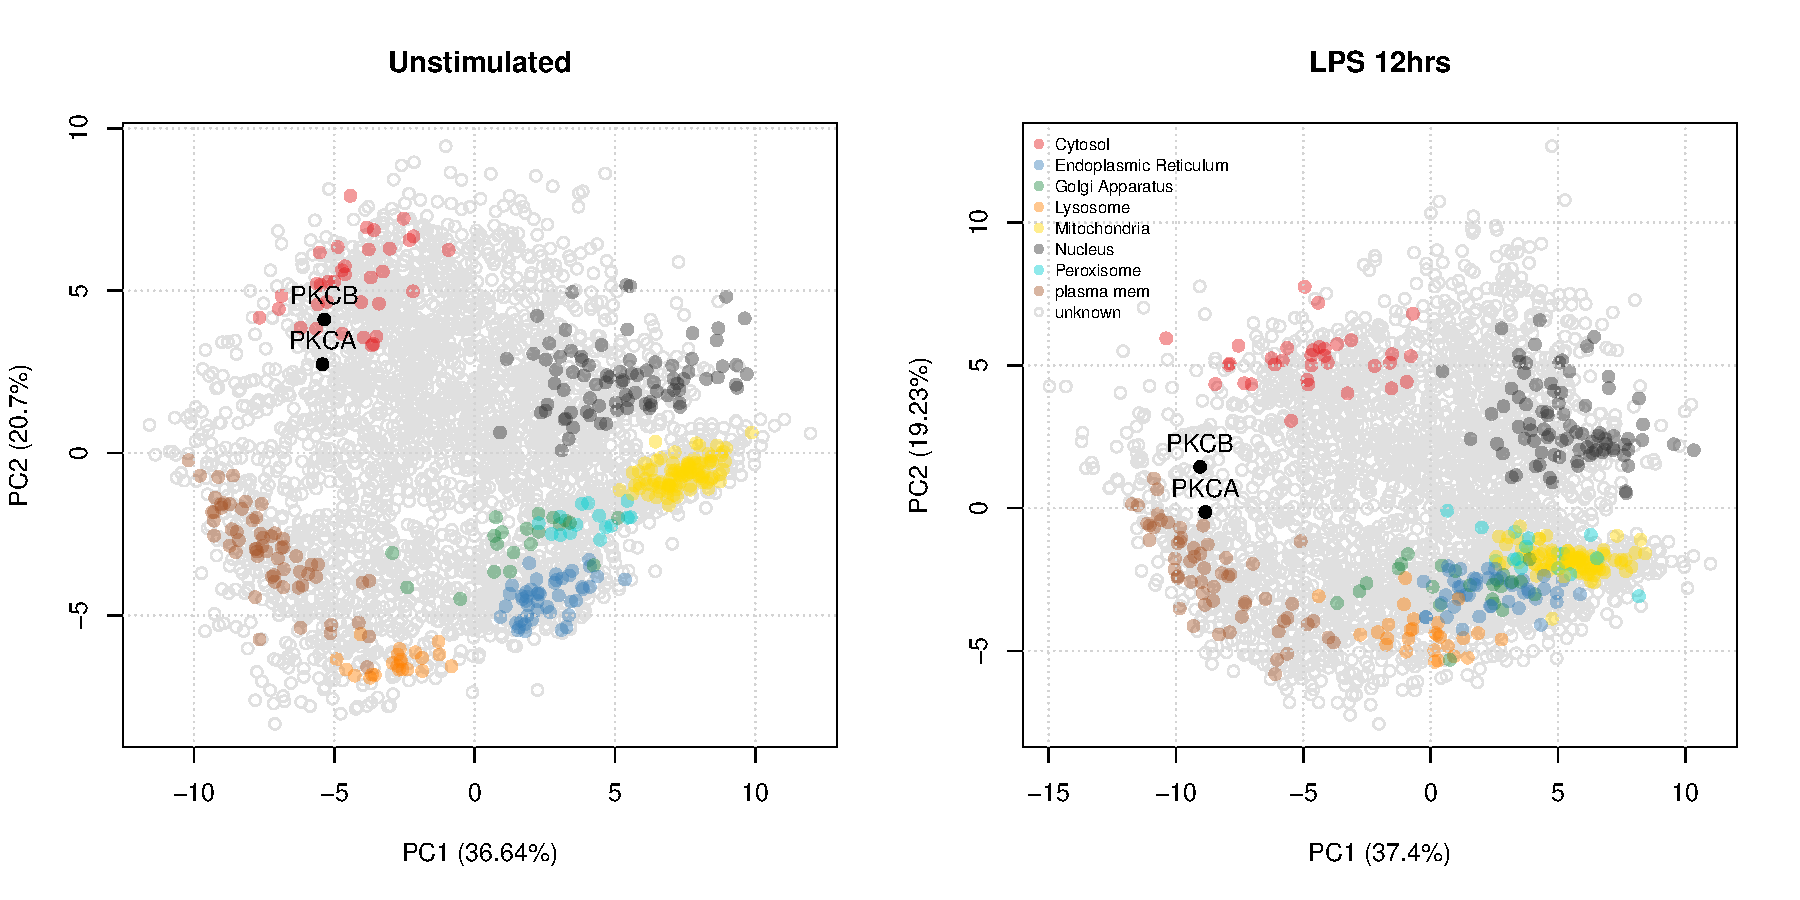
\includegraphics[width=\linewidth]{./figs_local/lps-pkc.pdf}
    \caption{Relocation of Protein Kinase C $\alpha$ and $\beta$ from the
      cytosol to the plasma membrane, \textbf{driving maturation into
        a differentiated macrophage phenotype}.}
  \end{figure}
\end{frame}

\begin{frame}
  \begin{figure}[h]
    \centering
    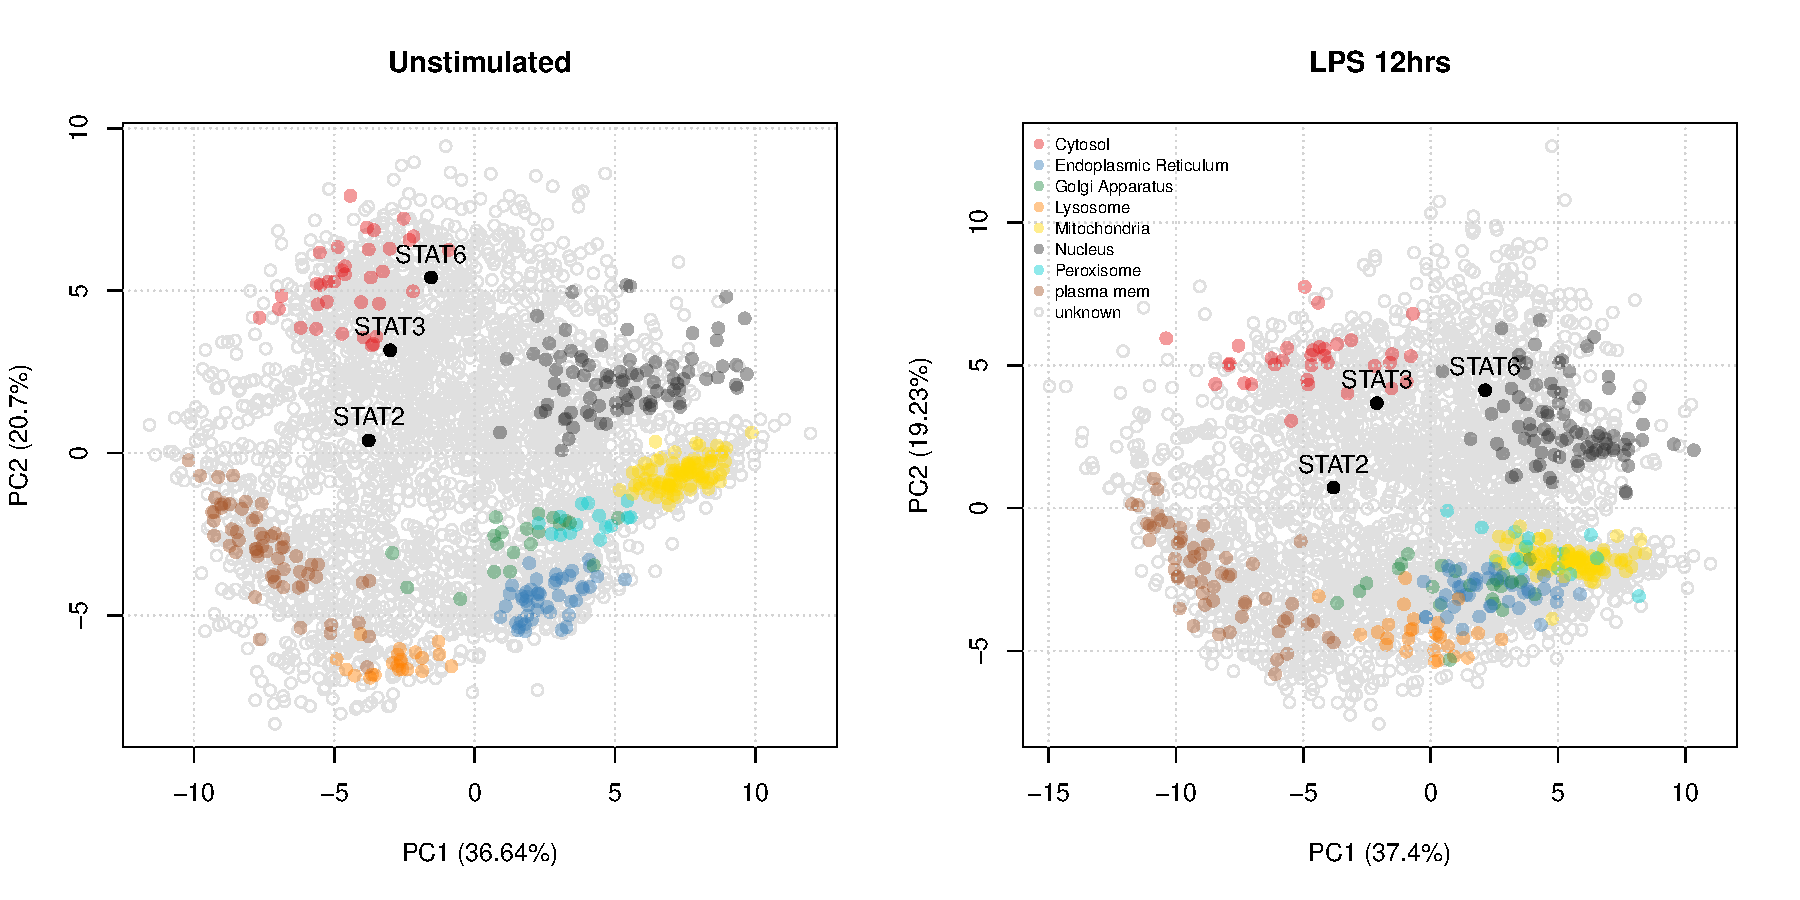
\includegraphics[width=\linewidth]{./figs_local/lps-stat.pdf}
    \caption{Relocation of Signal transducer and activator of
      transcription 6 (STAT6) from the cytosol to the Nucleus,
      \textbf{activating anti-bacterial and anti-viral-like
        response}. Validated by microscopy and see also
      \cite{Chen:2011}.}
  \end{figure}
\end{frame}


\section{Computational infrastructure}

\begin{frame}{}

  Beyond the figures\footnote{... which are all reproducible, by the way.}

  \bigskip

  Software: \textbf{infrastructure}
  (\href{http://bioconductor.org/packages/MSnbase}{\texttt{MSnbase}},
  \cite{Gatto:2012}), \textbf{dedicated machine learning}
  (\href{http://bioconductor.org/packages/pRoloc}{\texttt{pRoloc}},
  \cite{Gatto:2014a}), \textbf{interactive
    visualisation}\footnote{\url{https://lgatto.shinyapps.io/christoforou2015/}}
  (\href{http://bioconductor.org/packages/pRolocGUI}{\texttt{pRolocGUI}},
  \cite{pRolocGUI}) and \textbf{data}
  (\href{http://bioconductor.org/packages/pRolocdata}{\texttt{pRolocdata}},
  \cite{Gatto:2014a}) for spatial proteomics.

\end{frame}



\begin{frame}[allowframebreaks]{References}
  \tiny
  \bibliographystyle{plainnat}
  \bibliography{spatial_proteomics,bib2}
\end{frame}


\begin{frame}
  \begin{block}{Acknowledgements}
    \begin{itemize}
    \item \textbf{Mr Oliver Crook} and \textbf{Dr Lisa Breckels},
      Computational Proteomics Unit, Cambridge (machine learning,
      algorithms, software).
    \item \textbf{Dr Sebastian Gibb} and \textbf{Dr Johannes Rainer}
      (software).
    \item \textbf{Prof Kathryn Lilley} \textit{et al.}, Cambridge
      Centre of Proteomics and \textbf{Dr Claire Mulvey}, Cancer
      Research UK Cambridge Institute (spatial proteomics)
    \item \textbf{Funding}: BBSRC, Wellcome Trust
    \end{itemize}
  \end{block}



  \begin{center}
    Slides: \url{https://zenodo.org/record/1180393} \\

    \bigskip
    \textbf{Thank you for your attention}
  \end{center}

\end{frame}

\include{add}

\end{document}
